\section{Code Design}
In the following sections to come, we will go over the design and rationale of the choices
we made during the development of the code. In several instances, we will describe 
classes and methods that we believe are beneficial for the reader. Moreover, we will
give examples of the code such that the reader can become more
comfortable with the syntax. As a road map, Figure \ref{fig.phd_design} shows a high level view of the code. As it can be seen, the code consists of six core components:
simulation, integration, temporal control, geometric computation, core fluid
computation and optional fluid computation. This categorization, has lead the code
to be flexible enough to allow modifications without heavily disrupting other
portions of the code. Furthermore, each component may composed of one or more
subcomponents. In the next sections we will go into detail of each component and subcomponent.
\begin{figure}
    \begin{center}
        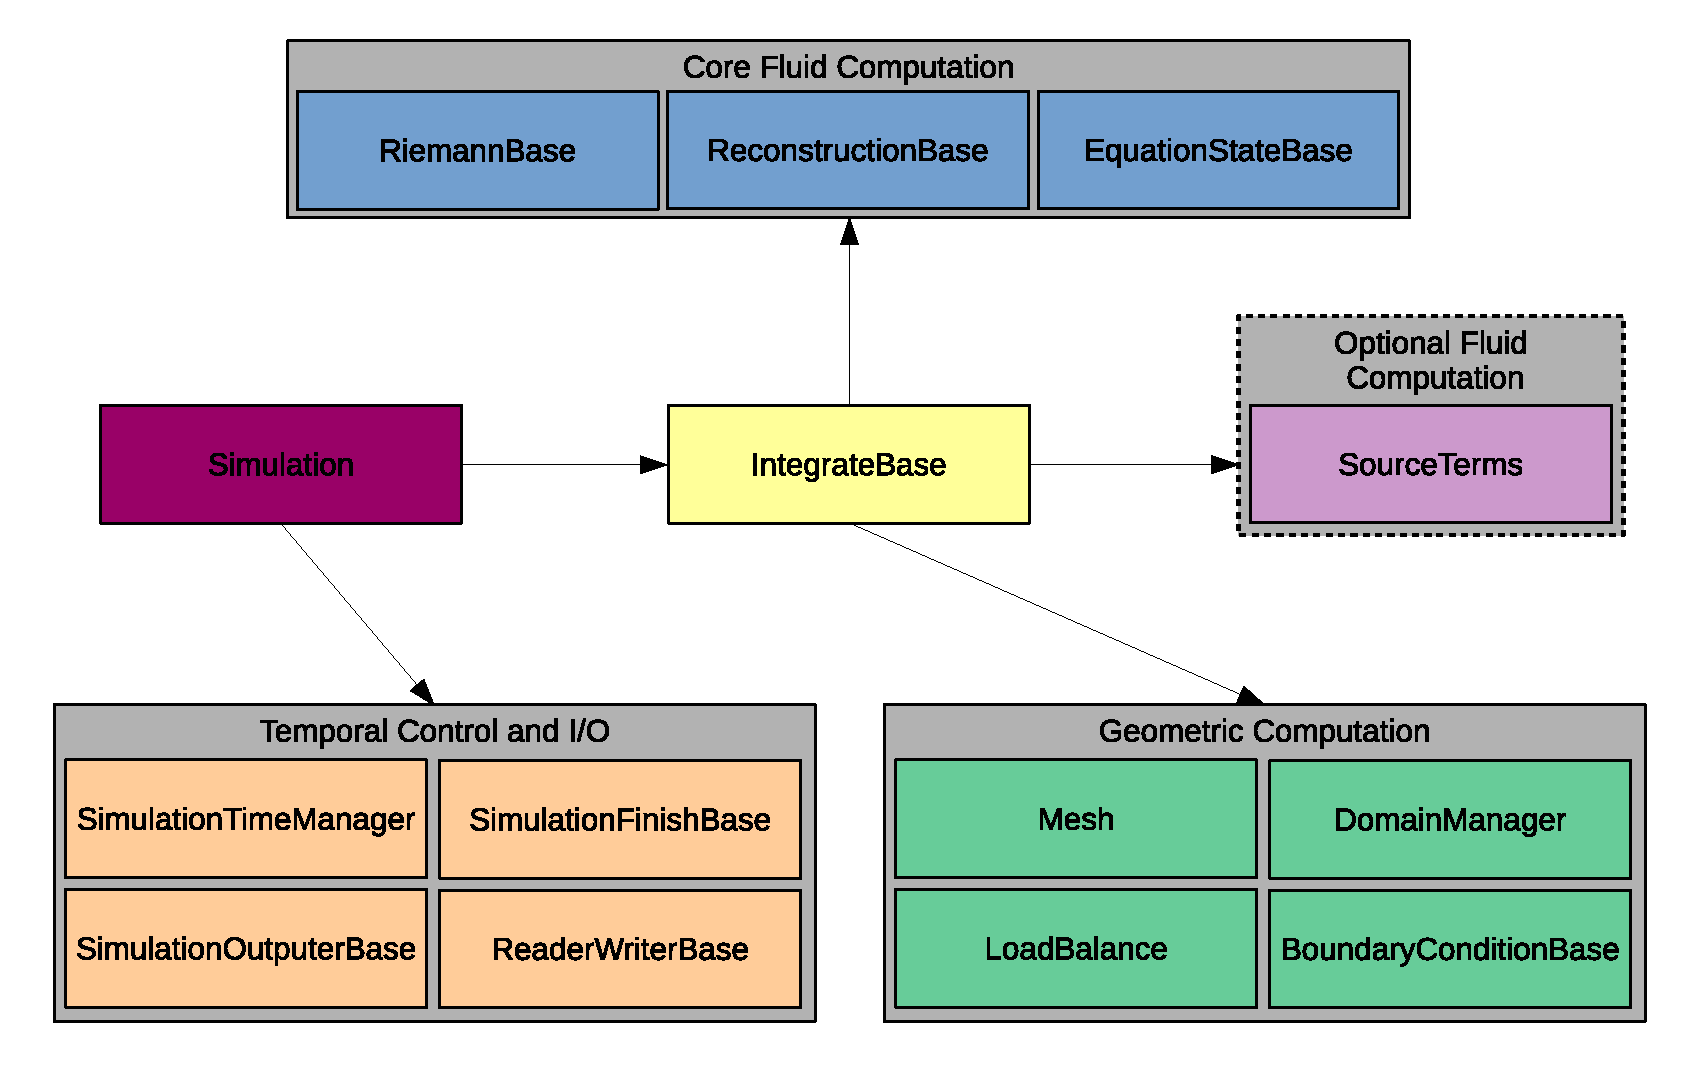
\includegraphics[width=0.8\textwidth]{figures/phd_chart.eps}
        \caption{High level view of the the \texttt{phd} code. The code is compromised of six core components
        that have been color coded. Each component is comprised of one or more classes. Each class
        represent a designated computation. Classes that have ``Base'' in their
        name can be easily modified through inheritance.}
        \label{fig.phd_design}
    \end{center}
\end{figure}

\subsection{Overall Class Design Considerations}
Before we go into specific details of the code, we outline some of the over arching
traits that are common throughout the code. Specifically we will describe field registration,
inheritance and data structures.

\subsubsection{Field Registration}
Form our past experience, we have found out that one of the challenging problems in maintaining codes
is that of adding new fields. There are many reasons why to add new fields, for example,
an implementation of new physics module (MHD, radiation, chemistry etc.) or adding a passive scalar
to track some portion of the fluid or modification of an existing algorithm that needs an auxiliary
field which has not been stored. In any case, the addition of a new field can be challenging
if the computation has been hard coded or the data structures, for example C structs, do not
allow for the addition of new fields. For this reason, we adopted a data structure
that allows registration of fields (see Section~\ref{sec.carraycontainer}). In this manner
fields can be easily added in the future.

From these considerations we will see a common thread with our classes, most have a method
for field registration or addition:
\begin{itemize}
	\item \lstinline{register_fields()} add fields to the simulation.
    \item \lstinline{add_fields()} add fields to self by inspecting current simulation fields.
\end{itemize}
For registration, the class usually inspects the particle data structure and creates fields
necessary for the simulation. As an example, gravity registers the acceleration to the particles
in the proper dimension. In this manner, we don't have unnecessary fields during the simulation
(3D fields for 2D runs). Likewise, for addition of fields the class usually inspects the
particle data structure and proceeds to register the proper fields internally. For example, gravity 
registers internally tree moment fields with the proper dimension.

Since any number of fields can be registered, we have also allowed the ability to group
fields by names. This has been extensively used to group collections of fields such as
primitive and conservative fields. This has allowed to easily retrieve groups of fields
that can computed as a whole.

\subsubsection{Class Dependencies}
Another source for future problems is when an algorithm depends on another. For example
our gravity tree solver depends on our load balance implementation. If the algorithms
are designed concurrently, then proper consideration is taken account on how they will
interact with one another. However, because of the development of new algorithms or experimentations, 
classes will eventually need to interact with others that where not originally designed for. In these
situations common options are to re-factor the algorithm or even rewrite the algorithm itself. Both 
methods can become cumbersome as the code develops and matures and changing one portion of the code 
may create a cascade of unwanted changes.

In our case we decided to write our classes as encapsulated computations (see Figure 
\ref{fig.phd_design}). This means we have
tried to segregate oure computations as independent tasks with interactions between each other
defined through an Application Programming Interface (API). For the most part, each computation
has a base class (i.e \lstinline{ReconstructionBase}, \lstinline{RiemannBase}, 
\lstinline{InetgrateBase} etc.) that
defines the methods it can perform. Moreover, the base class only serves as a template and
returns a warning if accessed. Thus, each implementation inherits the base class and defines
the actual computation. Further, if a method depends another class it has to be written in
such a way that it confines to the API. Therefore, our algorithms are designed to conform to an API
and any future development will have to abide by it.

\subsection{Serialization of classes and parameters}
\subsection{Particle Data Structures}
\subsubsection{Carray Class}
In choosing the underlying data structure several considerations where taken into account. First, the
data has to be accessible in \texttt{Python} and in \texttt{C}. Second, the data structure has to
accommodate several different data types. For this reason we chose a data structure that mimics
\texttt{Numpy} arrays, in the sense that the raw data is allocated in \texttt{C} and an interface exist that
manipulates the data in either \texttt{C} or \texttt{Python}. With this approach a decision had to be
made in the form of the raw data. Two choices where considered, either the data would
be held in structs or arrays. The benefit of structs would allow subfields of the data
be compact and allow easy implementations of passing and receiving data from other
processors in parallel runs. Further \texttt{Numpy} has an interface, that treats
arrays of structs as record \texttt{Numpy} arrays. However, this form was abandoned early on
as the sub-fields would have to be hard coded and would not allow the creation of
dynamic fields at run time. With this consideration, the raw data was chosen to be
\texttt{C} arrays. 

The exact implementation heavily depends on the \lstinline{Carray} class from the \texttt{pysph} code 
\citep{Ramachandran2016}. We have used this class as a starting point and have built functionality around
it. This class can be initialized in \texttt{Python} or \texttt{Cython} and the
interface closely resembles the list class of \texttt{C++} by allowing indexing and memory management. 
Further, \lstinline{Carray}s can return a \texttt{Numpy} array, allowing the user to use all \texttt{Numpy} 
functional (i.e. slicing and fancy indexing). Below is a simple example using a \lstinline{Carray}.
\begin{lstlisting}
import phd

# allocate carray of size 10 doubles
# and assign values
x = phd.DoubleArray(10)
for i range(len(x)):
	x[i] = i**2

x.append(3.21) # append value at the end of carray
x.resize(5)    # resize to 5 doubles

xnp = x.get_npy_array()      # numpy array reference
xnp[:] = np.arange(x.length) # numpy slice
\end{lstlisting}
In this example a \lstinline{Carray} is created with 10 doubles, then assigned values by indexing. Notice
that the length of the \lstinline{Carray} can be found by using the \lstinline{len()} function or the 
\lstinline{length} attribute. The \lstinline{Carray} then has a value appended to it followed by
a resizing of length of 5. Finally, the get \lstinline{npy_array()} is called returning a \texttt{Numpy}
array which allows the use of slicing. 

\subsubsection{CarrayContainer Class}
\label{sec.carraycontainer}
The use of Carrays allow to easily manipulate arrays of certain type of data. However, there are
many circumstances for the need of a collection of Carrays. For example the x, y, and z position
of a particle or the center of mass and moments of a node in the gravitational tree. Therefore,
another data structure has been implemented to facilitate the use of collection of Carrays. The data
structure is called a CarrayContainer and like the Carray it has many methods to manipulate the
underlying data. The CarrayContainer in some aspects mimics a python dictionary in the sense
that each carray can be retrieved by a string key.
\begin{lstlisting}
import phd
import numpy as np

carrys = {"x": "double", "y", "double"}

ca_con = phd.CarrayContainer(10, carrays)
size = ca_con.get_carray_size()
ca_con["x"][:] = np.random.rand(size)
ca_con["y"][:] = np.random.rand(size)

ca_con2 = phd.CarrayContainer(5, carrays)
size = ca_con.get_carray_size()
ca_con["x"][:] = np.random.rand(size)
ca_con["y"][:] = np.random.rand(size)

ca_con.append(ca_con2)
ca_con.remove(np.array([1, 3, 9])
\end{lstlisting}
Most of the routines of Carrays have been extended to CarrayConatiner to operate on
all Carrays in the Container. Further the container has routines to subset, remove, paste
and add values to certain elements.

\subsection{Simulation Class}
The \lstinline{Simulation} class is the main driver for advancing the solution in time
and coordinating outputs to disk and terminal. The two most important methods of this
class are listed below
\begin{itemize}
    \item \lstinline{solve()}: advance \lstinline{IntegrateBase} to its final state while
        outputting all necessary information. 
    \item \lstinline{compute_time_step()}: aggregate all time steps and enforce the smallest.
\end{itemize}
From its inception, the class was designed to be independent of the solvers. This was 
accomplished by distinguishing state computation and state advancing methods. For example,
\lstinline{IntegrateBase} can only perform a computation at a given temporal state 
(see Section~\ref{sec.integrator} for details) while \lstinline{Simulation} can
dictate when and the number of computations. Thus, \lstinline{Simulation} controls the
time advancement independently of the equations being solved. As of writing three integrators
exist, however, adding a new integrator is relatively straightforward.

During the course of a simulation the class is responsible to schedule outputs and
determined if the simulation has completed. Simulation outputs and termination are 
designated by the \lstinline{SimulationOutputerBase} and \lstinline{SimulationFinisherBase} 
classes respectively (see Section~\ref{sec.outputters} for details). At the end of every time
step the class calls \lstinline{compute_time_step()} to modify the current time step and
output any necessary data by cycling through all outputters. Likewise, at the beginning of
the time step the class cycles through all \lstinline{SimulationFinisherBase} classes 
in search for a termination signal.

Lastly, the simulation class also controls logging information (see Section~\ref{sec.logging}
for details). 
Log information is currently printed to the terminal and saved to a log file. The simulation class 
allows the ability to pick how much information should be printed and saved. In parallel runs, the 
root processor takes responsibility for writing to the log file and displaying to terminal.


% Temporal Control and I/O
%~~~~~~~~~~~~~~~~~~~~~~~~~~~~~~~~~~~~~~~~~~~~~~~~~~~~~~~~~~~~~~~~~~~~~~~~~~~~~~~~~~~~~~~~~~~~~~~
\subsection{Temporal Control and I/O}
\subsubsection{Reader/Writer Class}
To allow the code to output different data formats, we have implemented 
a \lstinline{ReaderWriterBase} class. This gives the freedom to the user
in what format should the particle information be saved in. Likewise, this
allows that data to be read in any format. The standard api of the 
\lstinline{ReaderWriterBase} is listed below:
\begin{itemize}
	\item \lstinline{read()} read data in a specific format.
    \item \lstinline{write()} write data in a specific format.
\end{itemize}
With such a framework, new formats can be easily implemented. Further, this
allows a simple way to create a front end to read data from another simulation.

Although this framework facilitates the option to save data in different formats,
we believe this framework has more general capabilities. Since the \lstinline{ReaderWriterBase}
has accessed to the integrator, any component of the simulation and be considered for
output. Moreover, analysis can be performed ouputing information that techniqua

\begin{lstlisting}
...
class EnergyTracker(ReaderWriterBase):
	def write(self, base_name, output_directory, integrator):
   		particles = integrator.particles
        
   		# compute square velocity
        v2 = particles["velocity-x"]**2 + particles["velocity-y"]**2
        if len(particles.carray_named_groups["position"]) == 3:
        	v2 += particles["velocity-z"]**2
            
        # calculate kinetic and potential energy of system    
        kinetic = (0.4*particles["mass"]*v2).sum()
        potential = 0.5*(particles["mass"]*particles["potential"]).sum()
        
        message = "Energy values: Kinetic %.2E Gravity %.2E" % (kinetic, potential)
        phdLogger.info(message)
\end{lstlisting}

\subsubsection{Outputer and Finisher Class}
\label{sec.outputters}

The code has been desinged to handle arbitrary signals for outputing data
and completion of the simulation. This has been achieved by introducing the
\lstinline{SimulationOutputerBase} class for output and
\lstinline{SimulationFinisherBase} class for completion.

At the end of every
time step (\lstinline{SimulationOutputerBase} includes the beginning and ending
of the simulation) a call to all registered outputers and finishers is
performed. In each call the class has complete control of the integrator. Thus
the classes can inspect the time, time step, iteration, particle data, flux data,
reconstruciton data etc. This allows for a general conditions instead of hard
coded ones. Further this opens the door to allow conditions

the options are plentiful and we hope to make large of use in the next
revision of the code.

In the case of \lstinline{SimulationOutputerBase} a writer is registered with it.

In this section we show, some what trivial but highlights the main points, an example of
how to create an outputter and finisher. For our example, we use the sedov problem from 
section cite. We are interested to output all time steps once the shock has reached
a density $\rho=2$ and remains less than $\rho=3$. Of course in this situation one may
use the analytical solution to extrapolate when such values would occur. However that
assumes the shock track exactly. In our scenario we let the simulation do the work
for us.

First we begin by defining an outputter with the objective to start outputing
all data once the density value of $\rho=2$ has been reached (see code excerpt). This
is accomplished by inheriting \lstinline{SimulationOutputerBase} and modifying
\lstinline{check_for_output} and \lstinline{modify_timestep}. For over writing
\lstinline{check_for_output}, we check is the the outputter is the main loop state
and if the max density is greater than \lstinline{density_min}. Moreover, there
is no need to change the time step, therefore, it is left unaltered.


\begin{lstlisting}
...
class OutputSedovDensity(SimulationOutputerBase):
    def __init__(self, density_min, base_name="density_output",
                 counter=0, pad=4, **kwargs):
        super(OutputSedovDensity, self).__init__(base_name, counter, pad, **kwargs)
        self.density_min = density_min 

    def check_for_output(self, simulation):
        """Return True to signal the simulation has reached
        sedov interval to ouput data."""
        integrator = simulation.integrator
        state = simulation._state == SimulationTAGS.MAIN_LOOP
        output_sedov = integrator.particles["density"].max() >= self.density_min:

        if state and output_sedov:
            return True
        return False

    def modify_timestep(self, simulation):
        """Return consistent time step."""
        # not modifying
        return simulation.integrator.dt

\end{lstlisting}
At this point our data will be outputted until the simulation is finished. To
create a finisher at the moment when density has reached $\rho_{\mathrm{max}}$
we create a new class \lstinline{SedovDensityFinisher}. This class inherits
\lstinline{SimulationFinisherBase} and one needs to define the \lstinline{finished}
method. In our case we need only to compare our max density values with
$\rho_{\mathrm{max}}$.
\begin{lstlisting}
...
class SedovDensityFinisher(SimulationFinisherBase):
    def __init__(self, density_max, **kwargs):
        self.density_max = density_max

    def finished(self, simulation):
        """Return True to signal the simulation is finished
        if reached max iteration number.
        """
        if simulation.integrator.particles["density"].max() >= self.density_max:
            return True
        else:
            return False

\end{lstlisting}

Although are example was simplistic, we hope that it shows the flexibility and power
what the outputters and finishers may achieve.  

\subsubsection{Logging}
\label{sec.logging}
Event logging during a simulation is performed through the python 
\texttt{logging}\footnote{\url{https://docs.python.org/2/library/logging.html}} library. The library has 
many capabilities but for our intentions we have focused on displaying and storing messages related to the
state of the simulation. To that end, we use one logger called \lstinline{phdLogger}. This 
logger can be imported to any file and used to log any information of interest.

For our purposes, the logger has four levels of logging. They are listed below:
\begin{itemize}
	\item debug: detailed information or diagnosing.
    \item info: working as expected.
    \item success: a successful completion. 
    \item warning: unexpected result that may lead to future problem.
\end{itemize}
The log levels have been listed in order of inclusion. Meaning if ``warning'' is chosen, then all messages
types are logged. However if ``info'' is chosen only messages of type ``debug" and ``info'' or logged.
At runtime the log level and file to store the messages can be specified through the 
\lstinline{Simulation} class.

As an example we show a simple usage of the logger below:
\begin{lstlisting}
import logging
phdLogger = logging.getLogger("phd")
...
phdLogger.info("Starting kinetic energy calculation")
kinetic_energy = particles["mass"]*(particles["velocity-x"]**2 + particles["velocity-y"]**2)

if kinetic_energy.sum() > 0:
	phdLogger.debug("Kinetic energy greater than zero")
\end{lstlisting}
In this example we import the logger and print out a messages related to the calculation of the
kinetic energy. It is important to note that this example is true if run in serial or parallel. The logger
has been modified such that logging information and storage is always handled by the root processor.

\subsection{Integrator Class}
\label{sec.integrator}
To advance the the state of a fluid to a specific time, a suitable integration
scheme must be provided. Although we have laid out the details of the MUSCL-Hancock scheme
in section cite, in practice, many schemes are available with different degrees of 
strengths and weaknesses. Therefore, we found it necessary to have an implementation
that allows the ability to easily switch from integration schemes. To this end, we have
created the \lstinline{IntegrateBase} class which is responsible to advance the state
of the system by one time step. In this way, a simulation is viewed as a series of calls
to \lstinline{IntegrateBase} by the \lstinline{Simulation} class.
Note we say system, not the Euler equations. This
distinction is made because the \lstinline{IntegrateBase} is not limited to the Euler
equations and, in principle, can be used to implement other equations. As an example,
we have implemented a gravitational N-body solver in this framework. We find
this framework to be versatile, allowing the user to chose from different schemes
and allowing the ability to quickly create new schemes for experimentation.
Currently we have implemented a static and moving mesh MUSCL-Hancock and a leap
frog integrator.

To implement an integrator, the \lstinline{IntegrateBase} must be inherited. Below
is the \lstinline{IntegrateBase} api:
\begin{itemize}
    \item \lstinline{before_loop()} perform any needed initialization or initial computations. 
    \item \lstinline{compute_time_step()} compute current state time step.
    \item \lstinline{evolve_time_step()} evolve the state of the system by one time step.
    \item \lstinline{after_loop()} perform any clean up or needed final computations.
\end{itemize}
For each integrator implementation one must define each method from the api. The integrator
has references to all the computation classes as well as state attributes (iteration
counter, time step, and time). The most
involved method is the \lstinline{evolve_time_step()} which defines the equations
and method to be used. For clarity, we shown two integrator examples below. The first
is an implementation of a non moving mesh MUSCL-Hancock integrator.
\begin{lstlisting}
def evolve_timestep(self):
    """Solve the compressible gas equations."""

    phdLogger.info("StaticMeshMUSCLHancock: Starting integration")

    # build left/right states at each face in the mesh
    self.reconstruction.compute_gradients(self.particles, self.mesh,
            self.domain_manager)
    self.reconstruction.compute_states(self.particles, self.mesh,
            self.equation_state.get_gamma(), self.domain_manager, 0.5*self.dt,
            self.riemann.boost)
    self.compute_source("primitive")

    # solve riemann problem, generate flux
    self.riemann.compute_fluxes(self.particles, self.mesh, self.reconstruction,
            self.equation_state)

    # update conservative from fluxes
    self.mesh.update_from_fluxes(self.particles, self.riemann, self.dt)
    self.compute_source("flux")
    self.compute_source("compute")

    self.compute_source("conservative")
    self.domain_manager.update_ghost_fields(self.particles,
            self.particles.carray_named_groups["conservative"],
            True)

    # convert updated conservative to primitive
    self.equation_state.primitive_from_conservative(self.particles)
    self.iteration += 1; self.time += self.dt
\end{lstlisting}
As it can be seen the method is a series of core computations. The method
begins by calculating the gradients followed by computing the left/right
states for the riemann solver. Once the fluxes are calculated they are used
to update the fields. Sprinkled in are calls to source terms, if any.
Finally the ghost particles, iteration counter and
time are updated and the system is ready for the next computation.


% Geometric Computation
%~~~~~~~~~~~~~~~~~~~~~~~~~~~~~~~~~~~~~~~~~~~~~~~~~~~~~~~~~~~~~~~~~~~~~~~~~~~~~~~~~~~~~~~~~~~~~~~
\subsection{Geometric Computation}
\subsubsection{Mesh Class}
The mesh class \lstinline{Mesh} is responsible for all geometric computations relating
to the particle cell. For example the class computes the cells volume and center of mass.
The class works in tandem with the \lstinline{DomainManager} to build the mesh.
Once constructed the mesh class register geometric fields that will be needed during
the simulation.

The tessellation algorithm section is performed through \lstinline{build_geometry()}.
It works withe the \lstinline{DomainManger} building the mesh in rounds. In the first
round all local particles are added to the tessellation, at this point there are no
ghost particles. Particles that have infinite volume or that have radius that intersect
with other processor boundaries, in parallel, or the simulation domain are flagged. Then the 
\lstinline{DomainManager} is called creating the necessary ghost particles. The mesh is
updated with the ghost particles and process is repeated. This process continues until
all particles have a finite volume and all neighbors have been accounted for.

With the tessellation complete, cell values are computed. This entail calculating
cell neighbors, volumes, center of masses, face area vectors etc. The information
regrading to the faces of each cell is stored an attribute \lstinline{faces}. In this
data structure, each column is a face. For each face entry there exists references to
the two particles that define the face. For each particle the neighbor information
is reference through faces. In this way, when a particle wants all of its neighbors
it first request all the faces relating to its cells. Then for each face, the neighboring
particle can be retrieved.

Once the flux have calculated, it is the responsibility of the mesh to use the fluxes
to update the values of the cells. This was chosen as the equation of update involves
geometric terms. Further this allows a framework to allow different structured meshes
(spherical and cylindrical). Since all geometric quantities are regulated to the mesh

\subsubsection{Domain Manager}
Our \lstinline{DomainManager} class is designed to handle information associated with
the domains of the simulation. We consider a domain to be the spatial region where the computation
is performed. In serial, this is the entire spatial region of the simulation.
In parallel, this is the spatial region associated with each processor. 
In this way, for the most part, our domains are isolated computations and when
data is needed from neighboring domains they are requested through the \lstinline{DomainManager}.

The \lstinline{DomainManager} was initially designed to contain the limits and dimension of
the problem. As development continued it became natural that the \lstinline{DomainManager} would
encompass the boundary condition, ghost particle information, and exchange of data across boundaries.
At its current state, the \lstinline{DomainManager} only supports communication of ghost particle data
and does not support the general forms of data communication
(i.e reduction, gathers, broadcast etc). We plan in the next revision to implement an api that
performs these task. In doing so, we would remove strict dependence on MPI functions and only
work through the \lstinline{DomainManager}.

%\subsubsection{Internal Boundary Particle Sharing}
In parallel, particles are decomposed into a disjoint set of spatial domains
with each domain mapped to a unique processor. The construction
of the global Voronoi mesh is then delegated to the construction of a disjoint set
of local Voronoi meshes. For the set of local constructions to be consistent
with the global mesh, the appropriate boundary particles must be 
communicated across domains.

Interior ghost particles, are particles formed from neighboring domains and are used to
connect local meshes together. Their creation is handled by the \lstinline{DomainManager}
through the \lstinline{create_interior_ghost_particles()} method. This method
creates interior ghost particles by inspecting the search radius of
each local particle. If a particles search radius overlaps with a processor
boundary then it is flagged and a corresponding ghost particle is created and exported to that processor.
The search method is made possible by the \lstinline{DomainManager}s ability to query
all domains through geometrical searches. Care is taken such that no duplicates are created through the 
whole process. After each particle is inspected, ghost particles are communicated and then the
mesh is allowed to updated itself. This procedure is repeated until particles are no longer flagged.

%\subsubsection{Particle Motion}
After a flux update, the particles are allowed to move. Depending on initial particle position and
velocity a particle may leave its processor or the simulation domain. In either case, the 
\lstinline{DomainManager} is responsible for the destintation of the particle.

%\subsubsection{Data Communication}
After the creation of ghost particles, in parallel simulations, supplemental data has to be communicated. 
For example, the center of mass may not be computed locally because its neighbors may not exist locally.
This is because our implementation of ghost particles only to guarantees all neighbors of local
particles. Certainly we could of opted to import all neighbors of ghost particles but instead we have 
decided to communicate that information instead. Thus, the \lstinline{DomianManager} records all information
associated with a ghost particle. This allows ghost particles to be easily updated with any data. These
operations are implemented through \lstinline{update_ghost_fields()} and 
\lstinline{update_ghost_gradients()}


When a particle leaves the simulation domain in serial or parallel the \lstinline{DomainManager}
flags that particle and then applies the boundary condition. For reflective boundaries the particle is not
allowed to leave and for periodic boundaries the particle is wrapped back into the domain. If the simulation
is in parallel the \lstinline{DomainManager} exports the particle to the correct processor and removes
it from the local particle container. If a particle leaves its processor patch the \lstinline{DomainManager}
will query all domains and find the correct domain for export.

\subsubsection{Boundary Condition}
Similar to interior ghost particles, exterior ghost particles are used to
complete local meshes. However, exterior ghost particles are not from neighboring
domains but instead are created through a boundary condition. To allow for different
boundary condition we have created \lstinline{BoundaryConditionBase} that interacts
with \lstinline{DomainManager}. The api is listed below:
\begin{itemize}
	\item \lstinline{create_ghost_particle()} create ghost particle from flagged particle.
    \item \lstinline{migrate_particles()} for particles that have left the domain, apply
    appropriate boundary condition.
    \item \lstinline{update_gradients()} apply boundary condition to ghost particle gradients.
    \item \lstinline{update_fields()} apply boundary condition to ghost particle fields.
\end{itemize}
Through this api, any boundary condition may be implemented. The boundary condition does not have
to be uniform in each dimension. Mixed boundaries or even problem specific boundaries are allowed
in this framework. Furthermore, the api allows the boundary
condition to modify particle motion and field data. In this way, we have extracted all boundary
information from the \lstinline{DomainManager}.

Currently, we have two implementations of boundary conditions, reflective and periodic.
In the reflective case, the flagged particle is mirrored across each boundary edge of the
simulation. If an intersection occurs, a ghost particle is created with its normal velocity flipped.
In the serial case, the ghost particle is added directly to the particle data container. In parallel, the 
ghost particle is then further inspected for intersection of neighboring processors. The ghost particle
is then placed in a communication to be exported to each flagged processor. For the periodic case
the procedure is similar, with the exception that particle is periodically shifted
instead of being mirrored.

\subsubsection{Load Balance}


% Core Fluid Computation
%~~~~~~~~~~~~~~~~~~~~~~~~~~~~~~~~~~~~~~~~~~~~~~~~~~~~~~~~~~~~~~~~~~~~~~~~~~~~~~~~~~~~~~~~~~~~~~~
\subsection{Core Fluid Computation}
\subsubsection{Riemann Solver}
The fluxes at each face of the mesh is constructed by the \lstinline{RiemannBase} class.
As a common thread with all of our computation classes, the base class defines the api.
The api is straight forward with only two methods to define:
\begin{itemize}
	\item \lstinline{riemann_solver()} solve for fluxes at each interface.
    \item \lstinline{compute_time_step()} compute hydro time step.
\end{itemize}
The \lstinline{compute_time_step()} is optional since the base class has a default
CFL constrained time step calculation. However the option is there if a particular 
solver implementation needs to modify it. Furthermore, the base class defines a 
method for the fluxes to be transformed back into the lab frame. This allows,
for the most part, to implement a solver without worrying about the details of
rotating and boosting back into the lab frame. As of time of writing, we have
implemented the HLL, HLLC, and Exact Riemann solvers.

\subsubsection{Reconstruction}
Once the mesh is created, cell center values need to be reconstructed to cell center faces
in order to calculate the fluxes. The interface to implement a reconstruction
scheme is dictated by the \lstinline{ReconstructionBase} class which has the following api:
\begin{itemize}
	\item \lstinline{compute_gradients()} calculate the gradients of the fields for each particle.
    \item \lstinline{add_spatial()} add gradients to expansion.
    \item \lstinline{add_temporal()} add time derivatives to expansion.
\end{itemize}
The api embodies a general deconstruction of eq. into three building blocks. First, is the
calculation of the spatial derivatives (i.e gradients) by \lstinline{compute_gradients()}.
In this call the derivatives are computed through a specified scheme. For example, the gradients can be 
calculated by the least square approach \citep{Pakmor2016} or through geometrical properties 
\citep{Springel2010}. With the derivatives calculated cell center values can then be extrapolated spatially
(\lstinline{add_spatial()}) or temporally (\lstinline{add_temporal()}). In this manner the
user has complete control of the terms in the expansion.This is important to note, as many integrator 
schemes make use of the reconstruction several times in Runge-Kutta solver variants (i.e \cite{Pakmor2016} 
and \cite{Duffell2011}).

\subsection{Equation of State}
Due to the implementation of the reconstruction and Riemann solvers, primitive fields
must be computed. The computation of primitive fields requires an equation of state. 
Since there are multiple formulations of an equation of state we have 
decided to implement an API through the \lstinline{EquationStateBase} class. The methods
are listed below:
\begin{itemize}
    \item \lstinline{conservative_from_primitive()}: compute conservative fields from primitive.
    \item \lstinline{primitive_from_conservative()}: compute primitive fields form conservative.
    \item \lstinline{sound_speed()}: compute the sound speed of the fluid.
    \item \lstinline{get_gamma()}: compute the ratio of specific heats.
\end{itemize}
The \lstinline{EquationStateBase} is responsible for converting the fields from conservative
to primitive and vice versa. Furthermore, the equation of state can calculate the sound
speed of the fluid. We have found this formulation to adequately remove the details of the
state of the fluid from other calculations.

Currently the \lstinline{EquationStateBase} is simplistic. However, in the next revision we plan
to extend its functionality. This is because a chemistry scheme is being developed. With an
added chemistry solver, additional species must be tracked and depending the equation of state
these fields.

% Optional Fluid Computation
%~~~~~~~~~~~~~~~~~~~~~~~~~~~~~~~~~~~~~~~~~~~~~~~~~~~~~~~~~~~~~~~~~~~~~~~~~~~~~~~~~~~~~~~~~~~~~~~
\subsection{Optional Fluid Computation}
\subsubsection{General Source Terms}
The inclusion of source terms has been implemented through a general source
\lstinline{SourceTermBase} with methods listed below:
\begin{itemize}
    \item \lstinline{apply_primitve()}: modify primitive variables.
    \item \lstinline{apply_conservative()}: modify conservative variables.
    \item \lstinline{apply_flux()}: modify flux terms.
    \item \lstinline{compute_source()}: calculate source components.
    \item \lstinline{compute_time_step()}: calculate time step from source term.
\end{itemize}
This formulation was chosen after some considerable experimentation. One of the
earlier attempts was a registration process. In this scenario a source term
would link any computation to class method. This information was stored
in a dictionary inside \lstinline{Simulation} and at runtime each class method
was over written using Pythons decorator scheme. Although, this scheme makes
use of more advance programming methods we found that this implementation was
not easy to discern. Moreover we found that this method left to much ambiguity
to the source terms, allowing . Instead we
found this current implementation to be more understandable and easier to
generalize.

The api listed above are the mandatory methods to be defined for any source
term. In general, we write an interface for each given source term. In this
way if the integrator changes only the api has to be updated leaving
the core of the source term unaltered. This also allows to easily implement
third party libraries as source terms, chemistry or radiation for example.
Once the methods have been defined the class is registered to 
\lstinline{Simulation} class and will be invoked at the appropriate parts
during the computation.

\subsubsection{Gravity}
For a more concrete example of how to include a source term we highlight the
pieces used to include self gravity. Our self gravity is a tree based implementation
named \lstinline{GravityTree}. Its main routine is \lstinline{walk()} which is the
calculation of gravitational accelerations from the current position of the particles.
To include this as a source term we created a new class called \lstinline{SelfGravity}
which inherits \lstinline{SourceTermBase}. As discussed in section, gravity alters
the momentum and primitive values.
\begin{lstlisting}
...
cdef class SelfGravity(MUSCLHancockSourceTerm):
    ...
    cpdef apply_primitive(self, object integrator):
        # loop over each face in the mesh 
        for m in range(integrator.mesh.faces.get_carray_size()):
            ....
            # add gravity to velocity
            for k in range(dim):
                vl[k][m] += 0.5*dt*a[k][i]
                vr[k][m] += 0.5*dt*a[k][j]

        # add gravity acceleration from particle
        for i in range(integrator.particles.get_carray_size()):
            ...
                for k in range(dim):
                    # update momentum
                    e.data[i] += 0.5*dt*mv[k][i]*a[k][i]

                    # update energy 
                    mv[k][i] += 0.5*dt*mass.data[i]*a[k][i]

    cpdef apply_conservative(self, object integrator):
        ...
        # add gravity acceleration from particle
        for i in range(integrator.particles.get_carray_size()):
            ...
                for k in range(dim):
                    # update momentum
                    mv[k][i] += 0.5*dt*mass.data[i]*a[k][i]

                    # update energy 
                    e.data[i] += 0.5*dt*mv[k][i]*a[k][i]
\end{lstlisting}
